\documentclass[swedish,a4paper,twopage=no,12pt]{scrbook}


\usepackage{geometry}
\usepackage{nopageno}
\areaset[0cm]{18cm}{26cm}

%\linespread{0.85}

%\usepackage{bookman}
\usepackage[T1]{fontenc}
\usepackage[utf8]{inputenc}
\usepackage{babel}
\setcounter{tocdepth}{3}

\clubpenalty = 10000 
\widowpenalty = 10000

\setlength\parskip{\baselineskip}
\setlength\parskip{\medskipamount}

%\setlength\parindent{0pt}
%\setlength{\unitlength}{1cm}
%\addtolength{\textheight}{2cm}

\usepackage{bookman}

\usepackage{graphicx}
\usepackage{ae}
\usepackage{aecompl}
\usepackage{amssymb}
\usepackage{amsmath}

\usepackage{tikz}


\begin{document}

%\begin{center}
%Nomogram för bakning Celsius till Fahrenheit.\\
%\end{center}
%\begin{tikzpicture}[scale=1.1] %[xscale=1.4,yscale=1.3]
%
%
%% densitet
%\draw[thick] (0,0) --(15.4,0); 
%\node at (16,0.4) {$^\circ C$};
%\node at (16,-0.4) {$^\circ F$};
%
%
%\foreach \x in {50,100,...,300}{
%	\node at (\x*0.06-2.8,0.6)  {\x};  
%	\draw[ultra thick] (\x*0.06-2.8,0.2) -- (\x*0.06-2.8,0);
%}
%\foreach \x in {75,125,...,275}{
%	\node at (\x*0.06-2.8,0.6)  {\x};  
%	\draw[thick] (\x*0.06-2.8,0.2) -- (\x*0.06-2.8,0);
%}
%
%\foreach \x in {150,200,...,550}{
%	\node at (\x*6/180-3.8667,-0.6)  {\x}; 
%	\draw[ultra thick] (\x*6/180-3.8667,-0.2) -- (\x*6/180-3.8667,0);
%}
%\node at (0.2,-0.6)  {120}; \draw[ultra thick] (0.2,-0.2) -- (0.2,0);
%\node at (10.7,-0.3) {\small{437}}; \draw[thick] (10.7,-0.1) -- (10.7,0);
%\node at (13.7,-0.3) {\small{527}}; \draw[thick] (13.7,-0.1) -- (13.7,0);
%
%
%\end{tikzpicture}
%
%\begin{tikzpicture}[scale=1.1] %[xscale=1.4,yscale=1.3]
% för feber Celsius till Fahrenheit.\\
%\vspace{20mm}\\
%
%
%
%
%\draw[thick] (0,0) --(15.4,0); 
%\node at (16,0.4) {$^\circ C$};
%\node at (16,-0.4) {$^\circ F$};
%
%\foreach \x in {36,37,...,42}{
%	\node at (\x*15/6-89.8,0.6)  {\textbf{\x}}; 
%	\draw[ultra thick] (\x*15/6-89.8,0.2) -- (\x*15/6-89.8,0);
%}
%\foreach \x in {36.1,36.2,...,42}	\draw[thick] (\x*15/6-89.8,0.1) -- (\x*15/6-89.8,0);
%\foreach \x in {36.5,37.5,...,41.5}   \draw[thick] (\x*15/6-89.8,0.2) -- (\x*15/6-89.8,0);
%
%\foreach \x in {97,98,...,107}{
%	\node at (\x*15/10.8-134.24,-0.6) {\textbf{\x}};
%	\draw[ultra thick] (\x*15/10.8-134.24,-0.2) -- (\x*15/10.8-134.24,0);
%}
%
%\foreach \x in {97.1,97.2,...,107}{
%	\draw[thick] (\x*15/10.8-134.24,-0.1) -- (\x*15/10.8-134.24,0);
%}
%
%\foreach \x in {97.5,98.5,...,107}{
%	\draw[thick] (\x*15/10.8-134.24,-0.2) -- (\x*15/10.8-134.24,0);
%}
%
%%subfebril
%
%\draw[green,  very thick] (36.3*15/6-89.8,0.03) -- (37.5*15/6-89.8,0.03);
%\draw[green,  very thick] (36.3*15/6-89.8,-0.03) -- (37.5*15/6-89.8,-0.03);
%
%\draw[cyan,  very thick] (37.5*15/6-89.8,0.03) -- (38*15/6-89.8,0.03);
%\draw[cyan,  very thick] (37.5*15/6-89.8,-0.03) -- (38*15/6-89.8,-0.03);
%
%\draw[yellow,  very thick] (38*15/6-89.8,0.03) -- (40*15/6-89.8,0.03);
%\draw[yellow,  very thick] (38*15/6-89.8,-0.03) -- (40*15/6-89.8,-0.03);
%
%\draw[magenta,   thick] (39*15/6-89.8,0.04) -- (40*15/6-89.8,0.04);
%\draw[magenta,   thick] (39*15/6-89.8,-0.04) -- (40*15/6-89.8,-0.04);
%
%
%\draw[magenta, very thick] (40*15/6-89.8,0.03) -- (41*15/6-89.8,0.03);
%\draw[magenta, very thick] (40*15/6-89.8,-0.03) -- (41*15/6-89.8,-0.03);
%
%
%\draw[red,  very thick] (41*15/6-89.8,0.03) -- (42*15/6-89.8,0.03);
%\draw[red,  very thick] (41*15/6-89.8,-0.03) -- (42*15/6-89.8,-0.03);
%
%
%\end{tikzpicture}

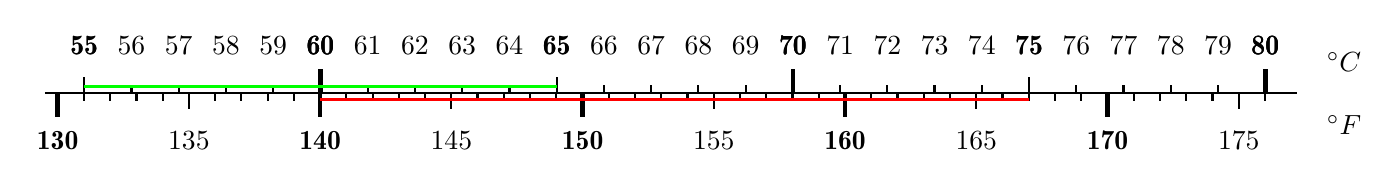
\begin{tikzpicture}[scale=1] %[xscale=1.4,yscale=1.3]


\draw[thick] (-0.5,0) --(15.4,0); 
\node at (16,0.4) {$^\circ C$};
\node at (16,-0.4) {$^\circ F$};

\foreach \x in {60,70,...,80}{
	\node at (\x*0.6-33,0.6)  {\text{\x}}; 
	\draw[ultra thick] (\x*0.6-33,0.3) -- (\x*0.6-33,0);
}


\foreach \x in {55,60,...,80}{
	\node at (\x*0.6-33,0.6)  {\textbf{\x}}; 
	\draw[thick] (\x*0.6-33,0.2) -- (\x*0.6-33,0);
}


\foreach \x in {55,56,...,80}{
	\node at (\x*0.6-33,0.6)  {\text{\x}}; 
	\draw[thick] (\x*0.6-33,0.1) -- (\x*0.6-33,0);
}

\foreach \x in {130,140,...,170}{
\node at (\x/3-43.67,-0.6)  {\textbf{\x}};
	\draw[ultra thick] (\x/3-43.67,-0.3) -- (\x/3-43.67,0);
}

\foreach \x in {135,145,...,175}{
\node at (\x/3-43.67,-0.6)  {\text{\x}};
	\draw[ thick] (\x/3-43.67,-0.2) -- (\x/3-43.67,0);
}

\foreach \x in {131,132,...,176}{
	\draw[thick] (\x/3-43.67,-0.1) -- (\x/3-43.67,0);
}


% beta amylase
\draw[green,  very thick] (55*0.6-33, 0.08) -- (65*0.6-33,0.08);
% alfa amylase
%\draw[cyan,  very thick] (60*0.6-33,0.03) -- (75*0.6-33,0.03);
\draw[red,  very thick] (60*0.6-33,-0.08) -- (75*0.6-33,-0.08);
%
%\draw[yellow,  very thick] (38*15/6-89.8,0.03) -- (40*15/6-89.8,0.03);
%\draw[yellow,  very thick] (38*15/6-89.8,-0.03) -- (40*15/6-89.8,-0.03);
%
%\draw[magenta,   thick] (39*15/6-89.8,0.04) -- (40*15/6-89.8,0.04);
%\draw[magenta,   thick] (39*15/6-89.8,-0.04) -- (40*15/6-89.8,-0.04);
%
%
%\draw[magenta, very thick] (40*15/6-89.8,0.03) -- (41*15/6-89.8,0.03);
%\draw[magenta, very thick] (40*15/6-89.8,-0.03) -- (41*15/6-89.8,-0.03);
%
%
%\draw[red,  very thick] (41*15/6-89.8,0.03) -- (42*15/6-89.8,0.03);
%\draw[red,  very thick] (41*15/6-89.8,-0.03) -- (42*15/6-89.8,-0.03);
%

\end{tikzpicture}


\end{document}

